This section is divided into two parts. In \autoref{sec:method-TreX}, we describe the T-reX program, and in \autoref{sec:method-casestudy}, we describe the methodology used to calculate the waste and material inventory footprints in a case study of five Li-ion batteries.

\subsection{T-reX}\label{sec:method-TreX}

\subsubsection{Computational framework}

Developed in the Python programming language, T-reX extends the \texttt{brightway LCA framework}, utilising the components \texttt{bw2data}, \texttt{bw2calc}, and \texttt{bw2io}~\citep{mutel2017brightway}. Additionally, the \texttt{wurst} package---which can deconstruct databases into a list of exchanges---is used to facilitate searching and data transformation at the exchange level (the individual supply chain flows)~\citep{mutel2017wurst}. Integration with the \texttt{premise} package~\citep{sacchi2022premise}---which integrates the projections of integrated assessment models (IAMs) into current LCA databases---enables the user to easily create and manipulate prospective LCA databases. T-reX is also compatible with \texttt{ActivityBrowser}~\citep{steubing2020activitybrowser}---an open-source graphical user interface for LCA---and after running T-reX, the manipulated databases and the `pseudo-LCIA' methods created by T-reX can be used in the project in the accustomed way. T-reX is installable via the Python Package Index (PyPI)~\citep{mcdowall2023T-reXpipy} and is fully open-source under the CC-0 licence. The full source code for T-reX is indexed on Zenodo~\citep{mcdowall2023T-reXzenodo} and under further development in the GitHub repository~\citep{mcdowall2024T-reXgithub}. T-reX is designed to be used with \texttt{ecoinvent} databases~\citep{ecoinvent2016version3}, but could be adapted to other databases by changing the search criteria. Currently, it has been tested with all available system models of \texttt{ecoinvent}versions 3.5--3.10.

T-reX can be used directly from the command line, or imported as a Python package, in which case, the user can access the individual functions and modules. In the simplest case, the user can run the program with the default settings, which will calculate the waste and material footprint of the \texttt{ecoinvent}database. The user can adapt the settings of T-reX as desired, to calculate alternative or additional waste and material inventory footprints, use a custom database, or a `prospective' database based on future scenarios by implementing the premise \texttt{premise} with one of T-reX's internal modules.

The supplementary material in \autoref{sec:supplementary} contains metadata of T-reX, along with a list of the constituent modules, a description of their functions, and a detailed computational workflow. Further details can be found in the GitHub repository and package documentation~\citep{mcdowall2024T-reXgithub, mcdowall2023T-reXdocs}.

\subsubsection{Functionality and purpose}

T-reX is a Python package that enables one to produce LCA databases---both current and prospective---that are manipulated to facilitate the calculation of waste and material inventory footprints in the supply chain of any activity in the same way as one would apply standard LCIA methods. We refer to the T-reX methods as `pseudo-LCIA' methods, as they represent an accounting of an activity's technosphere inventory without reference to impact modelling, as in standard LCIA.

If desired, prospective databases can be defined by the user or constructed with the projections of the integrated assessment models such as IMAGE~\citep{stehfest2014image} and REMIND~\citep{remind2020model}, which offer a range of options aligned with the Shared Socioeconomic Pathways (SSPs)~\citep{ssp2020ghg} and can be paired with a variety of mitigation scenarios.

The deconstruction of the databases by T-reX into lists of exchanges allows the relevant flows of material and waste to be identified and categorised by the search functions. The queries facilitating this are tailored to the specific database and the user can easily modify them to suit their needs. The categories defined in the configuration are used to create T-reX's `pseudo LCIA' methods that are indicators of aggregated technosphere demand. The exchange editing function of T-reX then takes each list of exchanges and appends to the relevant activity a copy of the technosphere exchange as a mirrored `pseudo-biosphere' exchange that matches the `pseudo-LCIA' method.

In the default configuration, there are 10 waste categories which are further divided by their unit of measurement (kilograms and cubic meters) to create a total of 20 waste methods. The waste categories include incineration, recycling, and total waste, and are listed in the supplementary material in~\autoref{sec:supplementary}. One advantage of T-reX is that it can identify `hidden' waste exchanges that would otherwise be `consumed' by a treatment process and not leave the technosphere. Since `waste is not a service'~\citep{guinee2021wasteisnotaservice}, a characterisation factor of -1 is applied to the waste footprint methods (except CCS exchanges), changing the perspective from `waste consumed by treatment' to `waste generated by the activity'.

In addition to the waste categories, T-reX can incorporate any number of material demand categories, the defaults being based on the EU Critical Raw Materials (CRM) list for 2023~\citep{eu2023crmstudy}, which contains 30 materials considered essential to the EU economy and also at risk of supply disruption. Especially valuable in the case of CRMs is T-reX ability to uncover and quantify these threads of background consumption, which can be inconspiciusly embededded in products or consumed in seemingly distant supply chain activities. The identity of the materials considered and their categorical groupings are easily customisable by the user, and in further materials of interest to the authors were added to the example Li-ion case study, including helium, electricity, petroleum, sand, water, and natural gas. The full list of 59 materials included in the default configuration is provided in the supplementary material in ~\autoref{sec:supplementary}.

The logic for the identification of material exchanges with T-reX differs from that used to identify waste exchanges in that the search queries are based on the names of the so-called relevant `market activities' for the material of interest rather than keywords in the exchange's name. A useful feature of T-reX is that, in cases where there are several markets for one material or material group, the program can aggregate these flows. For example, exchanges with markets for the rare-earth-elements (REEs) `market for cerium', `market for dysprosium', `market for erbium', etc.\ can be aggregated into a single indicator category for REEs. Similarly, the total demand for all critical raw materials (CRMs) can be calculated in the same manner.

% As presented in~\autoref{sec:intro-background},~\autoref{sec:intro-waste}, and~\autoref{sec:intro-material} of the introduction, there are some existing material demand methods in the standard LCIA method sets, including the CSI (which provides only an aggregated, abstracted endpoint in units of kg~Si~eq)~\citep{arvidsson2020csi} and the (deprecated) EDIP 2003 material use indicators (which provide endpoints in fundamental units)~\citep{hauschild2003edip}.

In these methods, the material demand is calculated based on the total mass that is extracted from the environment, thus, their focus is essentially solely on the mining-related exchanges that bring these materials from the biosphere into the technosphere.

T-reX, in contrast, uses accounting for material demand and waste generation based on exchanges solely within the technosphere. This offers a different perspective, allowing for the estimation of overall supply chain material demands that consider the entire life cycle of an activity, including non-direct impacts on the market such as co-production of other materials. Consider a demand for an activity containing a metal, for example; while the existing material use methods allow one to calculate the total mass of that metal that is extracted from the environment, T-reX can provide insight into the broader supply chain impacts of the demand for this metal. If the production of other materials is attributed to the production of this metal, these would appear as negative material demands in the T-reX results---supply chain pressure for one material can result in lessening of supply chain pressure for another. In the results of the Li-ion battery case study in \autoref{sec:results-casestudy}, we will see that this is indeed the case for nickel demand, which, in the final inventory because of such co-production, is counter-intuitively negative (due to co-production and substitution in the LCA system models) despite the presence of nickel in the final products.

% \subsubsection{Mathematical basis}

% \cbox{very nice formulae coming soon from LL hopefully}

\subsubsection{The workflow of T-reX}

The workflow of T-reX is divided into several modules, each performing a separate function. The modules are designed to be used in a particular order, but the user can also use them individually to perform specific tasks. The standard workflow is as follows:

\begin{enumerate}
    \item Configuration of waste and material exchange categorisation (optional)
    \item Generation of prospective LCA databases (optional)
    \item Database expansion---to create a list of all exchanges in the database
    \item Identification and categorisation of exchanges
    \item Creation of `pseudo-biosphere' databases
    \item Creation of `pseudo-LCIA' methods to calculate waste and material inventory footprints
    \item Exchange editing---whereby the technosphere exchange is mirrored as a `pseudo-biosphere' exchange
    \item Database verification---to ensure that T-reX has manipulated the database correctly
\end{enumerate}

This workflow creates a copy of the original \texttt{brightway} project containing the original biosphere database, a T-reX `pseudo-biosphere' database along with one or more manipulated technosphere databases that can be used to calculate the waste and material inventory footprints of activities in the same way as standard LCIA calculations.

An overview of the T-reX workflow is presented in \autoref{fig:methods-flowchart}. The supplementary material in \autoref{sec:supplementary} contains a more detailed computational flowchart.

\begin{figure}[H]
    \centering
    \caption{Workflow of T-reX. Application of T-reX to one or more LCA databases creates a \texttt{brightway} project with customised methods and activities that can be used to calculate waste and material inventory footprints of the activity's supply chain.}
    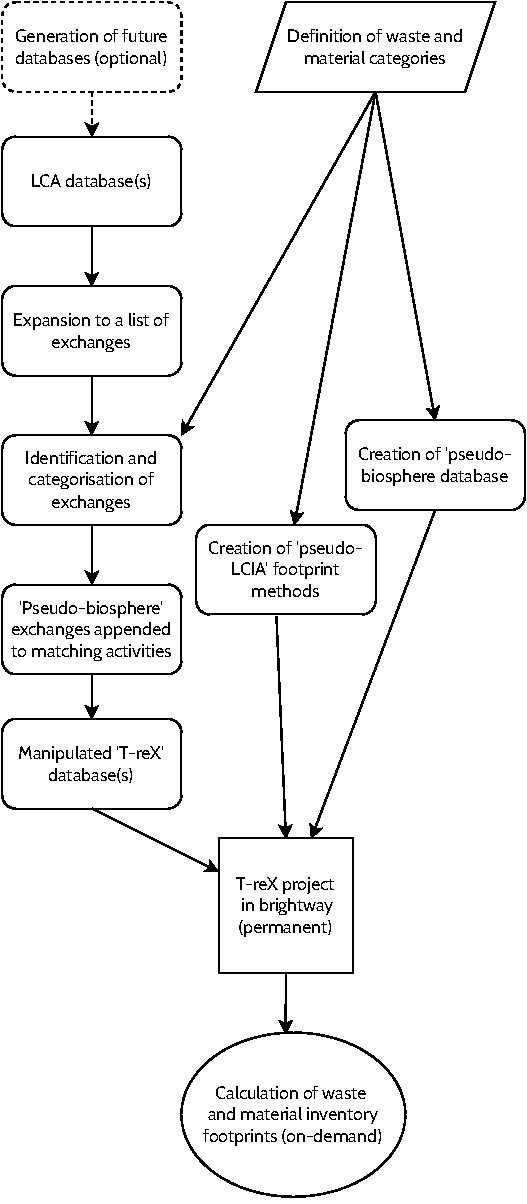
\includegraphics[width=14cm]{figures/T-reX_method.pdf}\label{fig:methods-flowchart}
\end{figure}


\subsection{Case study methodology}\label{sec:method-casestudy}

We investigated five types of Li-ion batteries, each represented by their unamended global market activities:
\begin{itemize}[itemsep=0pt]
    \item Li-ion, LFP, rechargeable, prismatic
    \item Li-ion, LiMn\(_2\)O\(_4\), rechargeable, prismatic
    \item Li-ion, NMC111, rechargeable, prismatic
    \item Li-ion, NMC811, rechargeable, prismatic
    \item Li-ion, NCA, rechargeable, prismatic
\end{itemize}

In addition to the waste and material inventory footprint methods created by T-reX, the following standard LCIA methods were applied for comparison:

\begin{itemize}[itemsep=0pt]
    \item ReCiPe 2016 v1.03, midpoint (I)
    \item EF v3.0 no LT
    \item EDIP 2003 no LT
    \item CSI 2020
\end{itemize}

The source of the life cycle inventory data for this case study was \texttt{ecoinvent}, version 3.9.1, with the `cutoff' attributional system model. Additionally, T-reX was used to create prospective database sets using the functionality of \texttt{premise} with the REMIND model and the baseline scenario SSP2 `middle of the road' with the following Representative Concentration Pathways (RCPs):
\begin{itemize}
    \item SSP2-base: representing an approximate 3.5°C increase in global temperatures to 2100
    \item SSP2-PkBudg500: representing the achievement of Paris climate goals, ca. 1.3°C increase to 2100
\end{itemize}

For each pathway, databases (at five-year time intervals) were created with \texttt{premise}~\citep{sacchi2022premise} and processed with T-reX for the period between 2020 and 2100.

\subsubsection{LCA calculations}
For each combination of activity, method, and database, a single score was calculated along with details of the top contributing processes. Additionally, for the T-reX methods, a contribution analysis was performed. This involved utilising the \texttt{bwa.compare\_activities\_by\_grouped\_leaves} function from the \texttt{brightway2\_analyzer} package~\citep{mutel2016brightway2analyzer}, a component of the \texttt{brightway} ecosystem. This function performs graph traversal on the impact matrix of the LCA object to a specified cutoff and groups the resulting leaves by their Cooperative Patent Classification (CPC) codes. This provides insight into the products and sectors in the supply chain of the activity that carry the most substantial responsibility for the final waste generation or material demand footprints.


